% (The MIT License)
%
% Copyright (c) 2022-2023 Yegor Bugayenko
%
% Permission is hereby granted, free of charge, to any person obtaining a copy
% of this software and associated documentation files (the 'Software'), to deal
% in the Software without restriction, including without limitation the rights
% to use, copy, modify, merge, publish, distribute, sublicense, and/or sell
% copies of the Software, and to permit persons to whom the Software is
% furnished to do so, subject to the following conditions:
%
% The above copyright notice and this permission notice shall be included in all
% copies or substantial portions of the Software.
%
% THE SOFTWARE IS PROVIDED 'AS IS', WITHOUT WARRANTY OF ANY KIND, EXPRESS OR
% IMPLIED, INCLUDING BUT NOT LIMITED TO THE WARRANTIES OF MERCHANTABILITY,
% FITNESS FOR A PARTICULAR PURPOSE AND NONINFRINGEMENT. IN NO EVENT SHALL THE
% AUTHORS OR COPYRIGHT HOLDERS BE LIABLE FOR ANY CLAIM, DAMAGES OR OTHER
% LIABILITY, WHETHER IN AN ACTION OF CONTRACT, TORT OR OTHERWISE, ARISING FROM,
% OUT OF OR IN CONNECTION WITH THE SOFTWARE OR THE USE OR OTHER DEALINGS IN THE
% SOFTWARE.

\documentclass{article}
\usepackage{../ppa}
\newcommand*\thetitle{Abstract Machines}
\newcommand*\thesubtitle{...}
\begin{document}

\plush{\innoTitlePage{5}}

\pptToc

\plush{\pptChapter[Turing]{Who Are Abstract Machines?}}

\pptSection{Definition}

An \emph{abstract machine} is a theoretical \emph{model} of computation.

Similar to a function, a machine receives \emph{inputs} and produces \emph{outputs} based on predefined \emph{rules}.

Abstract machines are ``machines'' because they allow \emph{step-by-step} execution of programmes. (really?)

They are ``abstract'' because they ignore many aspects of actual (hardware) machines.

An abstract machine is an \emph{intermediate language} with a small-step operational semantics.

\plush{}

\pptSection{Purpose}

``The implementation of a programming language consists of two
stages. The implementation of the compiler and the implementation of the abstract (virtual?) machine.
This is a typical divide-and-conquer approach.
From a pedagogical point of view, this simplifies the presentation and
teaching of the principles of programming language implementations.
From a software engineering point of view, the introduction of layers of
abstraction increases maintainability and portability.'' (\href{https://www.sciencedirect.com/science/article/abs/pii/S0167739X99000886}{1999})

\plush{}

\pptSection{Virtual Machines}

An abstract machine implemented in software is termed a \emph{virtual machine},
and one implemented in hardware is called simply a ``machine.''

\plush{}

\pptSection{LLVM}

LLVM (Low Level Virtual Machine) is a standard de-facto.

\pptPic{0.7}{llvm.png}

\plush{}

\plush{\pptChapter[Turing]{Turing Machine}}

Turing Machine was the first (1936) ... but not the simplest.

\pptPic{0.7}{turing.png}

For example, Emil Post's Machine is simpler.

\plush{}

\plush{\pptChapter[FSM]{Finite-State Machine}}

\plush{\pptChapter[SECD]{SECD Machine(s)}}

There are SECD (\textbf{s}tack, \textbf{e}nvironment, \textbf{c}ontrol, \textbf{d}ump),
CESK, CEK, CS, and maybe other abstract machines.

I like the CRM (\textbf{c}ontrol, \textbf{r}esults, \textbf{m}emory) machine explained by
\href{https://software-lab.org/people/Michael_Pradel.html}{Michael Pradel} in
\href{https://www.youtube.com/watch?v=YRfb2zDk_qs}{his YouTube course} about program analysis:
$\langle c, r, m\rangle$.

\begin{equation*}
\begin{split}
\langle \texttt{x} \mathrel{\texttt{:=}} 2 \times 3, \texttt{nil}, \{\} \rangle
  & \longrightarrow \langle \texttt{x} \mathrel{\circ} 2 \times 3 \mathrel{\circ} \mathrel{\texttt{:=}}, \texttt{nil}, \{ \}\rangle \\
  & \longrightarrow \langle 2 \times 3 \mathrel{\circ} \mathrel{\texttt{:=}}, \texttt{x} \mathrel{\circ} \texttt{nil}, \{ \}\rangle \\
  & \longrightarrow \langle \mathrel{\texttt{:=}}, \texttt{x} \mathrel{\circ} \texttt{6} \mathrel{\circ} \texttt{nil}, \{ \}\rangle \\
  & \longrightarrow \langle \texttt{nil}, \texttt{nil}, \{ \texttt{x} \mapsto 6 \}\rangle \\
\end{split}
\end{equation*}

\plush{}

\plush{\pptChapter{Semantic}}

This is our programming language that helps us draw on a canvas:


\begin{multicols}{2}
{\ttfamily
L 10, 20, 15, 23; \\
C 13, 13, 45; \\
L 5, 28, 15, 12;}
\par\columnbreak\par
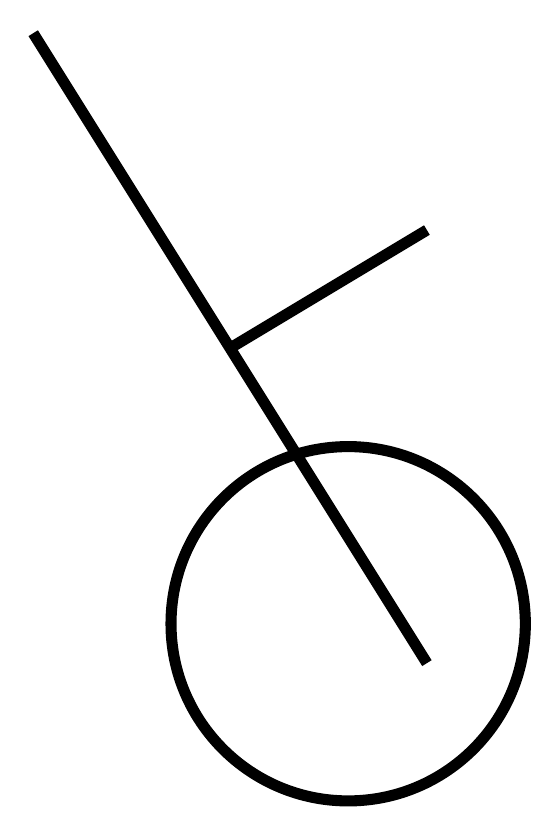
\begin{tikzpicture}[scale=5,line width=4pt]
\path[draw] (1, 2) -- (1.5, 2.3);
\path[draw] (.5, 2.8) -- (1.5, 1.2);
\node[circle,minimum height=4.5cm,draw] at (1.3, 1.3) {};
\end{tikzpicture}
\end{multicols}

Its semantic may be explained by the abstract machine with the following instruction set, which semantic is \textbf{obvious} to a reader:

{\ttfamily
MOVE x, y; DRAW; LOOP; BREAK; }


\end{document}
